\documentclass[11pt]{article}

\usepackage{graphicx}
\usepackage{graphics}
\usepackage{multicol}
\usepackage{epsfig,amsmath,amsfonts}

\makeatletter                                   % Make '@' accessible.

\oddsidemargin=0in                              % Left margin minus 1 inch.
\evensidemargin=0in                             % Same for even-numbered pages.
\marginparsep=0pt                               % Space between margin & text

\renewcommand{\baselinestretch}{1}              % Double spacing

\textwidth=6.5in                                % Text width (8.5in - margins).
\textheight=9in                                 % Body height (incl. footnotes)

\topmargin=0in                                  % Top margin minus 1 inch.
\headsep=0.0in                                  % Distance from header to body.
\skip\footins=4ex                               % Space above first footnote.
\hbadness=10000                                 % No "underfull hbox" messages.
\makeatother                                    % Make '@' special again.


\begin{document}

\fontfamily{cmss}                               % Make text sans serif.
\fontseries{m}                                  % Medium spacing.
\fontshape{n}                                   % Normal: not bold, etc.
\fontsize{10}{10}                               % 10pt font, 10pt line spacing 
\selectfont

\title{Mica High Speed Radio Stack}
\author{Nelson Lee, Philip Levis, Jason Hill}
\maketitle

\fontfamily{cmr}                                % Make text Roman (serif).
\fontseries{m}                                  % Medium spacing.
\fontshape{n}                                   % Normal: not bold, etc.
\fontsize{12}{12}                               % 12pt font, 12pt line spacing
\selectfont

\section*{Introduction}
This document describes the TinyOS networking stack released in TinyOS
1.0. This stack provides variable length packets and data-link level
synchronous acknowledgements at a 40Kb data rate; it only works on
mica motes. This document assumes the reader is familiar with nesC.

\section*{The Old Network Stack}

The pre-mica TinyOS networking components used a vertical protocol
stack. It roughly had this structure:

\small
\begin{verbatim}

       Application
            |
            V
       GENERIC_COMM
            |
            V
       AM_STANDARD
            |
            V
    CRCPACKETOBJ_SIGNAL
            |
            V
 SEC_DED_RADIO_BYTE_SIGNAL
            |
            V
           RFM

\end{verbatim}
\normalsize

This vertical layering made each component dependent on the
components directly above and below it, and allowed different
components (e.g. a non CRC packet) to be easily interchanged. However,
experience has shown that most of the interesting and important
functionality had to be encapsulated in {\tt SEC\_DED\_RADIO\_BYTE\_SIGNAL},
as only it could use the bit-level interface to the radio ({\tt RFM}).

For example, {\tt SEC\_DED\_RADIO\_BYTE\_SIGNAL} was responsible for the MAC
layer, packet start symbol detection, and data encoding/decoding:
three very separate pieces of functionality.

\section*{Introducing the New Radio Stack in nesC}

In nesC, configuration files link components together according to the
interfaces they use and provide.  The hierarchy that links
applications to the radio stack is as follows:

\small
\begin{verbatim}
        Application
            |
            V
        GenericComm (configuration ``/tos/system/'')
            |
            V
        AMStandard (module ``/tos/system'')
            |
            V
        RadioCRCPacket (configuration ``/tos/platform/mica'')
            |
            V
        MicaHighSpeedRadioM (module ``/tos/platform/mica'')
            |
     _______|___________________________________________
     |           |         |          |        |        |
     |           |         |          |        |        |
     V           |         V          |        V        |  
ChannelMonC.td   |  RadioTimingC.td   |   SlavePinC.td  |
                 V                    V                 V
          SpiByteFifoC.td        SecDedEncoding.td  RandomLFSR.td

\end{verbatim}
\normalsize

All componenents below {\tt RadioCRCPacket}, except for {\tt RandomLFSR}, are  
implemented in \\{\tt /tos/platform/mica}.


\section*{A Brief Overview}

Several components combine to form the network stack.

\begin{itemize}

\item {\tt MicaHighSpeedM} contains the logic and state at the
packet-level, and acts as a central controller for all of the
components below it. It does not communicate directly to hardware,
instead, it calls on other components to do so.

\item {\tt ChannelMonC} observes the radio at bit-level at 20kbps.  When the
stack is idle, it samples waiting for the preamble and start symbol.
When the stack is sending a packet and is in backoff, {\tt ChannelMon}
monitors the radio and signals idleDetect to {\tt MicaHighSpeeedM}.

\item {\tt SpiByteFifo} provides a byte-level abstraction to the radio.  In
essence, it uses the Serial Peripheral Interface (SPI) of the
ATmega103 processor to shift out bits to the radio when sending, and
shift in bits from the radio when receiving at 40kbps.  

\item {\tt SlavePinC} calls {\tt HPL} functions to flip the {\tt SlavePin} high and low.

\item {\tt RadioTiming} uses counters on the ATmega103 and input capture to sync a
receiver of a packet to the sender.

\item {\tt SecDedEncoding} provides a byte-level implementation of
encoding/decoding single error correction and double error detection.

\item {\tt RandomLFSR} returns a 16 bit random number. This is used by
{\tt ChannelMon} to determine the length of the backoff state in radio clock ticks.
\end{itemize}

\section*{Init/Idle}
The network stack is initialized by calling init() in
{\tt MicaHighSpeedRadioM}.  In turn, {\tt RandomLFSR} is initialized
and {\tt ChannelMonC}
is initialized.  {\tt RandomLFSR} initializes the seed from the ID of the mote
for the random number generator.  {\tt ChannelMonC} sets its {\tt CM\_waiting}
field to -1, sets the radio hardware to receiving, scales timer2 and
compare register2, clears the current counter value and enables
timer2's interrupt to go off every 200 clock ticks (200 clock
ticks/bit = 4MHz/20kbps).

Every time timer2's interrupt fires, {\tt TOSH\_SIGNAL(SIG\_OUTPUT\_COMPARE2)}
is called in {\tt ChannelMonC}. While the entire network stack is idle
({\tt MicaHighSpeedRadioM} has not accepted any packets and its {\tt
state} and {\tt send\_state}
are both {\tt IDLE\_STATE}), it shifts in the bit received into a buffer and
checks for the preamble. Preamble/start symbol detection will be
discussed in further detail below.

\section*{The new TOSMsg format}
The new structure of the {\tt TOS\_Msg} (the struct declaration can be found
in {\tt ``/tos/system/AM.h''}:

\begin{verbatim}
typedef struct TOS_Msg
{
  uint16_t addr;
  uint8_t type;
  uint8_t group;
  uint8_t length;
  int8_t data[TOSH_DATA_LENGTH];
  uint16_t crc;
  uint16_t strength;
  uint8_t ack;
  uint16_t time;
} TOS_Msg;
\end{verbatim}

It consists of an unsigned two byte field {\tt addr}, followed by
three unsigned single byte fields {\tt type}, {\tt group}, and {\tt
length} {\tt addr} specifies a moteID or the broadcast address ({\tt
0xffff}).  When the {\tt MicaHighSpeedRadioStackM} receives a packet,
the packet is passed to the AM level. If {\tt addr} is not the broadcast
address nor the address of the mote receiving the packet, the packet
is dropped.  The {\tt group} field specifies a channel for motes on a
network. If a mote receives a packet sent by a mote with a different
{\tt group} field, the packet is dropped at the AM level. The default
{\tt group}
is 0x7d. The {\tt type} field specifies which handler to be called at
the AM level when a packet is received. The {\tt length} field
specifies the length of the data portion of the {\tt TOS\_Msg}. Packets have
a maximum payload of 29 bytes.

The next field in the {\tt TOS\_Msg} struct is the {\tt data} portion. It
consists of an array of 29 bytes (as specified by
{\tt TOSH\_DATA\_LENGTH}). The unsigned two byte field {\tt crc}
follows. When sending, the CRC is incrementally calculated as each
byte of the packet is transmitted. The maximum length of a transmitted
{\tt TOS\_Msg} is 36 bytes ({\tt addr}(2 bytes) + {\tt type}(1 bytes)
+ {\tt group}(1 bytes) +
{\tt length}(1 bytes) + {\tt data}(29 bytes) + {\tt crc}(2 bytes = 36 bytes)). The {\tt
strength}, {\tt ack}, {\tt and time} fields are not transmitted; they
are meta-data about the packet.

The last three fields of {\tt TOS\_Msg} are the single unsigned byte {\tt
ack} field, the unsigned two byte {\tt strength} and unsigned two byte {\tt time}
fields.  The {\tt ack} is sent by the receiver, and set by the
sender. This is the mechanism that can provide reliability in the
stack. When the network stack finishes sending a packet, it will
return the {\tt TOS\_MsgPtr} to the application that issued the send
request, with the {\tt ack} field set to either 1 or 0.  If the field
is 1, the data link layer received an acknowledgement for the
packet. When a packet is received, the data link layer transmits an
{\tt ack} if the receiving mote is a valid destination for the packet:
({\tt rec\_ptr$->$addr == TOS\_LOCAL\_ADDRESS $\parallel$ rec\_ptr$->$addr ==
TOS\_BCAST\_ADDR}).  The {\tt strength} field of {\tt TOS\_Msg} is currently
unused, and the {\tt time} field stores an atomic capture of a 16-bit 4MHz
counter. 

\section*{Sending a Packet}
MicaHighSpeedRadioM contains two state variables, {\tt send\_state} and
{\tt state}.  When AMStandard hands down a {\tt TOS\_MsgPtr} to send,
MicaHighSpeedRadio's state must be {\tt IDLE\_STATE}.  If it is {\tt IDLE\_STATE}, then the
radio stack accepts the packet.  Its state changes and does not return 
until a packet is completely sent, which includes the reception of an
ack.

{\tt MicaHighSpeedRadioM} then calls {\tt macDelay}() in {\tt
ChannelMonC}.  {\tt macDelay} sets its {\tt CM\_waiting} field to a
random number.  {\tt CM\_waiting} specifies the number of {\tt
ChannelMonC} clock ticks (one {\tt ChannelMonC} clock tick is equal to
200 ATmega clock ticks at 4MHz) to wait for idle over the network.
This Backoff state, as described previously, ensures that a sender of
a packet in the network will not interfere with the transmission of
another sender's packet in the network. The random factor prevents
starvation.

Now, since {\tt ChannelMonC} is waiting for idleness in the network, each
call to \\
{\tt TOSH\_SIGNAL(SIG\_OUTPUT\_COMPARE2)} in {\tt ChannelMonC} decrements
{\tt CM\_waiting}.  When {\tt CM\_waiting} is equal to 1, it checks to see if 
during the past 12 {\tt ChannelMonC} clock ticks a single 1 bit was not
received (checking if {\tt CM\_search[0]} \& 0xfff == 0).  If so, it sets
{\tt CM\_waiting} to -1, disables timer2's interrupt (thereby disabling
{\tt ChannelMonC}) and signals {\tt MicaHigSpeedRadioM} that idleness was
detected on the network and that it may begin sending over the radio.
If activity was detected over the network, it sets {\tt CM\_waiting} to
another random number and continues waiting for idleness.  

It is important to note that while {\tt ChannelMonC} searches for idleness
over the network, it is simultaneously searching for a preamble. If a
preamble is detected, {\tt ChannelMonC} begins search for a start\_symbol.
This in effect switches the network into receive mode.  However,
when the network finishes receiving the packet or realizes that it
falsely detected a preamble, {\tt ChannelMonC} will return to {\tt IDLE\_STATE}
and resume its detection for an idle network to send the packet it
accepted to send. 

{\tt ChannelMonC} signals {\tt MicaHighSpeedRadioM} via the {\tt idleDetect} signal
handler that the network is idle and ready for transmission.
{\tt MicaHighSpeedRadioM} then calls on {\tt SecDedEncoding} to encode the first
byte of the {\tt TOS\_Msg}.  Each byte to be encoded results in three bytes
to be sent over the network. Hence, {\tt SecDedEncoding} signals
{\tt MicaHighSpeedRadioM} three times for each byte called to be
encoded. {\tt MicaHighSpeedRadioM} then activates {\tt SpiByteFifoC} to send the
first byte of the preamble/start symbol (char {\tt start[12]}), sets the
time field of the {\tt TOS\_Msg} to be sent ({\tt send\_ptr$->$time}), and begins crc
calculation with the first byte of the {\tt TOS\_Msg} to be sent
({\tt send\_ptr[0]}). {\tt MicaHighSpeedRadioM}'s {\tt msg\_length} field is also
calculated here. This value corresponds to the number of bytes to be
encoded and sent over the network excluding the crc. This calculation proceeds as follows: taking the
maximum number of unencoded bytes of a {\tt TOS\_Msg} that can be sent over
the network (36), subtracting the maximum length of the {\tt data} field
(29) and the {\tt crc} (2), adding the {\tt length} field of the
{\tt TOS\_Msg}, which specifies the number of bytes of the data array to be sent,
results in the number of bytes to be encoded and sent over the
network.  

{\tt SpiByteFifoC} holds at most two bytes at any time; the one that is
currently being sent, and the one that is waiting to be sent (uint8\_t
{\tt nextByte}). Being in {\tt IDLE} state corresponds to inactivity in
{\tt SpiByteFifoC}. When its buffer is free, its state is open, and when its buffer is
in use, its state is full.

{\tt SpiByteFifoC} receives a byte to send, and if it is
currently in its {\tt IDLE} state, which in this particular case it will be
since it was inactive before receiving the first byte of the start
symbol, it will accept the byte and signal to
{\tt MicaHighSpeedRadioM} that data is ready. {\tt SpiByteFifoC} also initializes
the SPI hardware, initializes and sets timer2 (modifying registers
{\tt TIMSK}, {\tt TCNT2}, {\tt OCR2}, {\tt TCCR2}), and sets the radio to transmit.

The hardware shift register used by the SPI is now configured to shift
in a bit from the radio every 100 clock ticks (100 ticks/bit =
4MHz/40kbps). After eight bits are shifted out of the {\tt SPDR} register
(data register of the SPI hardware) and sent over the network,
{\tt TOSH\_SIGNAL(SIG\_SPI)} in {\tt SpiByteFifoC} is called. The {\tt nextByte}
field of {\tt SpiByteFifoC} is then output to {\tt SPDR} and the hardware
continues shifting a bit out and sending it over the network at 40kbps
(1 bit every 100 clock ticks) for another group of eight bits. This is
the primary interface to the radio hardware for sending out
bits. Contrary to the old stack, there is no software layer that
communicates directly to radio hardware when sending.

To understand the following explanations on the intricacies of
{\tt MicaHighSpeedRadioM}, the distinction between ``calling send on a
byte'', ``sending a byte'', and ``signalling that a byte has been
sent'' must be fully understood.  {\tt SpiByteFifo} keeps a single byte
buffer. Calling {\tt send}() will place the byte in the buffer; the byte is
not immediately sent. {\tt SpiByteFifoC} can be in one of three states: {\tt IDLE},
when it not sending a byte, {\tt OPEN}, when it is sending a byte but its
buffer is open and can be used, and {\tt FULL}, when it is sending a byte
and has a byte in its buffer. When a byte has been sent, {\tt SpiByteFifoC}
signals a {\tt dataReady}() event. As there is a one byte queue, the
{\tt dataReady}() event for a given byte may not be the one immediately
following the {\tt send}() request. The calling component must keep track of
the {\tt send}() and {\tt dataReady}() counts to know which event is associated
with a specific byte.

When {\tt MicaHighSpeedRadioM} calls send on the first byte of the start symbol, its
state changes to {\tt TRANSMITTING\_START}. At each signal of {\tt dataReady}, it
calls send on the next byte of the start symbol.  After the tenth byte
of the preamble/start symbol has been sent, meaning {\tt dataReady} is
signaled with the tenth byte, {\tt MicaHighSpeedRadioM} calls send on the twelfth
and final byte of the preamble/start symbol and changes its state to
{\tt TRANSMITTING}.

When {\tt dataReady} is signaled for the eleventh byte of the
preamble/start symbol, \\
{\tt MicaHighSpeedRadioM} calls send on the
first encoded byte.  {\tt MicaHighSpeedRadioM} stores encoded bytes in
its 4 byte array encoded\_buffer. After send is called on two of the
three encoded bytes for a single byte of the {\tt TOS\_Msg}, {\tt
MicaHighSpeedRadioM} will call encode on the next byte of the {\tt
TOS\_Msg} to be encoded and buffered for sending. Using the field {\tt
tx\_count} as an index into {\tt send\_ptr} cast into a char*, the
byte pointed to will be the next byte encoded.

The field {\tt tx\_count} corresponds to the index of the next byte to be
encoded and buffered for sending. Let's use the application {\tt CntToRfm}
to illustrate how exactly {\tt MicaHighSpeedRadioM} behaves. The first
packet sent by {\tt CntToRfm} appears as follows:

\newpage

\begin{verbatim}
TOS_Msg:                       encoded bytes 
        addr    = 0xff          0x9b, 0x55, 0x55
                  0xff          0x9b, 0x55, 0x55
        type    = 0x4           0x52, 0xaa, 0x9a
        group   = 0x7d          0x48, 0x95, 0x59
        length  = 0x4           0x9b, 0x55, 0x55
        data    = 0x1           0x5b, 0xaa, 0x9a
                  0x0           0xa4, 0xaa, 0xaa
                  0x0           0xa4, 0xaa, 0xaa
                  0x0           0xa4, 0xaa, 0xaa
        crc     = 0xd9          0x58, 0x59, 0x69
                  0x2d          0x95, 0xa6, 0x59
\end{verbatim}

At each call to {\tt SpiByteFifo.dataReady}, {\tt send} is called on
the next encoded byte and {\tt enc\_count} is decremented. Therefore,
taking the first byte of the {\tt TOS\_Msg} (0xff), the order of
operations is as follows:

\begin{itemize}
\item {\tt tx\_count} is set to 1, and {\tt enc\_count} equals 3

\item {\tt SpiByteFifo.dataReady()} is signaled. Call {\tt SpiByteFifo.send}(0x9b) on the first encoded byte, decrement {\tt enc\_count} to 2

\item {\tt SpiByteFifo.dataReady()} is signaled. Call {\tt SpiByteFifo.send}(0x55) on the second encoded byte, decrement {\tt enc\_count} to 1.  To fill up the encoded buffer, call {\tt Code.encode(next\_data)} where {\tt
next\_data} is {\tt send\_ptr[tx\_count]}. Increment {\tt tx\_count}
to 2 and incrementally compute the crc ({\tt calc\_crc} = {\tt
add\_crc\_byte(next\_data, calc\_crc)}).

\item {\tt Code.encodeDone()} is signaled. Add the number of encoded bytes (3) to {\tt enc\_count}, to make it 4.

\item {\tt SpiByteFifo.dataReady()} is signaled. Call {\tt SpiByteFifo.send(0x55)} on the third encoded byte (the final encoded byte of the first data byte of the packet). Decrement {\tt enc\_count} to 3.

\item {\tt SpiByteFifo.dataReady()} is signaled. Call {\tt SpiByteFifo.send(0x9b)} on the fourth encoded byte (the first encoded byte of the second data byte of the packet). Decrement {\tt enc\_count} to 2.

\end{itemize}

This cycle repeats itself for each byte of the {\tt TOS\_Msg} that is
sent over the radio. In the instance of the {\tt dataReady} handler
that calls {\tt send} on the second to last byte of the encoded three
bytes of the second to last byte of the {\tt TOS\_Msg} to be sent (in
this case it would be the fifth to last encoded byte before the {\tt
crc}, 0xaa, refer to {\tt CntToRfm} example above), {\tt tx\_count} is
automatically changed to 34.  Therefore, independent of what {\tt
msg\_length} or the number of data bytes encoded and sent over the
network is, the {\tt crc} bytes will always be the last two byte
encoded and called {\tt send} on.

After the six bytes of the encoded {\tt crc} are called {\tt send} on,
{\tt MicaHighSpeedRadioM} changes its state to {\tt
SENDING\_STRENGTH\_PULSE}. The time from when {\tt
MicaHighSpeedRadioM} transitions from {\tt TRANSMITTING} to {\tt
SENDING\_STRENGTH\_PULSE}, to the time when it transitions from \\
{\tt SENDING\_STRENGTH\_PULSE} to {\tt WAITING\_FOR\_ACK}, two bytes
of 0xff are sent. As the name of the state suggests, a strength pulse
is sent. However, currently in the radio stack, the strength pulse is
used merely as a timing mechanism.

After the strength pulse is sent, during the transition from {\tt
SENDING\_STRENGTH\_PULSE} to \\
{\tt WAITING\_FOR\_ACK}, {\tt
SpiByteFifo.phaseShift()} is called. {\tt phaseShift} delays {\tt
SpiByteFifoC}, meaning {\tt SpiByteFifoC} pauses before resuming
shifting in bits from the radio.

Once {\tt MicaHighSpeedRadioM} enters the {\tt WAITING\_FOR\_ACK} state, it
transitions the radio to receive mode. {\tt SpiByteFifoC} continues to
signal {\tt dataReady} to {\tt MicaHighSpeedRadioM} in 800 clock tick intervals
(after 8 bits are shifted in), and the byte signalled (uint8\_t {\tt data}) corresponds to the byte heard
over the radio. {\tt MicaHighSpeedRadioM} listens for four bytes, and on the
last one, if the byte is equal to 0x55, then it sets the {\tt TOS\_Msg} {\tt ack}
field to 1, indicating the message sent was properly received. A
{\tt packetReceived} task is then posted, which sets {\tt MicaHighSpeedRadioM} to
{\tt IDLE\_STATE}, sets {\tt ChannelMonC} to {\tt IDLE\_STATE} and activates it to search for a preamble/start
symbol, and passes the sent packet to the AM layer with the {\tt ack} field and {\tt time} fields
set.

To summarize, the sender's interaction with the radio in the
{\tt CntToRfm} example is as follows:

\begin{verbatim}
                                bytes sent
                                -------------------
        addr    = 0xff          0x9b, 0x55, 0x55
                  0xff          0x9b, 0x55, 0x55
        type    = 0x4           0x52, 0xaa, 0x9a
        group   = 0x7d          0x48, 0x95, 0x59
        length  = 0x4           0x9b, 0x55, 0x55
        data    = 0x1           0x5b, 0xaa, 0x9a
                  0x0           0xa4, 0xaa, 0xaa
                  0x0           0xa4, 0xaa, 0xaa
                  0x0           0xa4, 0xaa, 0xaa
        crc     = 0xd9          0x58, 0x59, 0x69
                  0x2d          0x95, 0xa6, 0x59
        strength                0xff
        pulse                   0xff

        ---phase shift occurs---
        ---radio now set to receiving---
                                byte received 0x55
                                byte received 0x55
                                byte received 0x55
                                data = byte received (send_ptr->ack = (data == 0x55))
        DONE
\end{verbatim}


\section*{Receiving a Packet}
{\tt ChannelMonC} initiates the reception of a packet. When the radio stack
is initialized, \\
{\tt ChannelMon.startSymbolSearch} is called. This method
initializes {\tt ChannelMonC} to {\tt IDLE\_STATE} as described earlier in section
init/idle. Once {\tt ChannelMonC} detects a preamble, its state changes into
{\tt START\_SYMBOL\_SEARCH}, where it will shift in bits in search of a start
symbol. If a start symbol was not detected after 30 bits received, it
changes its state back to {\tt IDLE\_STATE}. If a start symbol was detected,
it signals {\tt MicaHigSpeedRadioM startSymDetect}.

In the {\tt startSymDetect} handler, {\tt MicaHighSpeedRadioM} changes its state
to {\tt RX\_STATE}, sets the {\tt time} field of the packet received to the current
time, trivially sets the {\tt strength} field of the packet to 0,
synchronizes the receiver ({\tt RadioTiming.getTiming}() and {\tt startReadBytes}(tmp)) to the sender and activates {\tt SpiByteFifoC} to
begin shifting in bits. Synchronization details can be found in
section Timing. 

{\tt SpiByteFifoC} is now configured to shift in bits sampled from the radio
once every 100 clock ticks, and signals {\tt dataReady} to
{\tt MicaHighSpeedRadio} after 8 bits have been sampled.

Now, each time {\tt dataReady} is called in {\tt MicaHighSpeedRadioM},
{\tt SpiByteFifoC} will call decode on the byte received and returned by
{\tt SpiByteFifoC}. {\tt SecDedEncoding} signals {\tt decodeDone} to {\tt MicaHighSpeedRadioM}
after three bytes have been called to be decoded. Therefore, most of
the logic for the receiver resides in the {\tt decodeDone} handler.

Many constants are used in the {\tt decodeDone} handler and they are
{\tt MSG\_DATA\_SIZE}, {\tt LENGTH\_BYTE\_NUMBER} and {\tt DATA\_LENGTH}. {\tt MSG\_DATA\_SIZE} is equal to 36,
the number of bytes of a {\tt TOS\_Msg} up to and including the {\tt crc} field.
{\tt LENGTH\_BYTE\_NUMBER} corresponds to the index of the {\tt length} field of
{\tt TOS\_Msg} when it is cast into a (char*).  {\tt DATA\_LENGTH} corresponds to
the size of the {\tt data} field of a {\tt TOS\_Msg}, which is currently set to
29.

The logic {\tt decodeDone} follows is nearly identical to the logic described
in the previous section for the sender of the packet. Each time a byte
is decoded, it is written into the buffer {\tt TOS\_Msg} ({\tt rec\_ptr}) using the
index {\tt rec\_count}. The field {\tt msg\_length}, corresponds to the number
of decoded bytes that should be received excluding the {\tt crc}. The
calculation for {\tt msg\_length} is the same as described in the previous
section, except that it cannot be calculated until it has received the
{\tt length} field of the packet being sent (if({\tt rec\_count} ==
LENGTH\_BYTE\_NUMBER)\{...\}). For the sender, {\tt msg\_length} can be calculated right away because the
length of the packet is passed as a paramter to the AM layer. 

Once {\tt msg\_length} bytes have been received and decoded, {\tt rec\_count} is
automatically set to 34 (if({\tt rec\_count} == {\tt msg\_length})\{...\}). This occurs because the next two bytes
decoded will be the {\tt crc}, and the index of the first byte of the {\tt crc} of {\tt rec\_ptr}, when
cast as a (char*), is 34.

As a note regarding CRC reception and calculation, each byte received
excluding the two {\tt crc} bytes is used to calculate the CRC. After the
{\tt crc} has been received, it is compared with the calculated CRC. If they
are the same, the {\tt crc} field of the {\tt TOS\_Msg} is set to 1 (if({\tt calc\_crc} ==
{\tt rec\_ptr->crc})\{ {\tt rec\_ptr->crc} = 1; ...\}). If not, {\tt rec\_ptr->crc} is set to
0.

If the received {\tt crc} and calculated CRC match, {\tt MicaHighSpeedRadioM}
checks if the address of the packet was either its own moteID or the
broadcast address. If so, it tells {\tt SpiByteFifoC} to send the ack
(0x55) and changes its state to {\tt ACK\_SEND\_STATE}. If not, a call to
{\tt SpiByteFifoC} send is not made.

After receiving the last decoded byte of the packet being sent, the
receiver will receive the first 0xff byte sent by the receiver during
the sender's {\tt SENDING\_STRENGTH\_PULSE} state. During this instance of
{\tt dataReady}, {\tt MicaHighSpeedRadio} will call {\tt SpiByteFifo.txMode}(), which
keeps {\tt SpiByteFifoC} active but changes the state of the hardware to transmit.

For the next five instances of {\tt dataReady}, either 0x00 or 0x55 is sent
over the wire: 0x00 if packet was corrupted or intended for a
different mote, 0x55 if the packet was received properly and addressed
to itself.

During the fifth instance of {\tt dataReady}, {\tt MicaHighSpeedRadioM}
deactivates {\tt SpiByteFifo} (call {\tt SpiByteFifo.idle}()), and posts a
{\tt packetReceived} task. The {\tt packetReceived} task sets the radio stack to
{\tt IDLE\_STATE}, signals to the AM layer that the packet was received, and
activates {\tt ChannelMonC} to search for a preamble/start symbol (call
{\tt ChannelMon.startSymbolSearch}). The purpose for this check, ``if(tmp !=
0) {\tt rec\_ptr} = tmp;'' in the {\tt packetReceived} task is because the AM layer
will return a {\tt TOS\_Msg} (tmp), but that {\tt TOS\_Msg} may be an application's buffer
and different than the buffer used to receive the packet. Therefore,
it is an established convention that the receive signal handler return
a free {\tt TOS\_Msg} for the radio stack to use for reception of another
packet when a packet was signalled upon reception. 

To summarize, the receiver's interaction with the radio in the
{\tt CntToRfm} example is as follows:
\begin{verbatim}
                                bytes received
                                -------------------
        addr    = 0xff          0x9b, 0x55, 0x55
                  0xff          0x9b, 0x55, 0x55
        type    = 0x4           0x52, 0xaa, 0x9a
        group   = 0x7d          0x48, 0x95, 0x59
        length  = 0x4           0x9b, 0x55, 0x55
        data    = 0x1           0x5b, 0xaa, 0x9a
                  0x0           0xa4, 0xaa, 0xaa
                  0x0           0xa4, 0xaa, 0xaa
                  0x0           0xa4, 0xaa, 0xaa
        crc     = 0xd9          0x58, 0x59, 0x69
                  0x2d          0x95, 0xa6, 0x59
        strength pulse          0xff

        ---radio now set to sending---
                                byte sent 0x55
                                byte sent 0x55
                                byte sent 0x55
                                byte sent 0x55
                                byte sent 0x55
        DONE
\end{verbatim}

\section*{Timing}
As discussed previously, there are two components that communicate
directly with radio hardware: {\tt SpiByteFifoC} and
{\tt ChannelMonC}. {\tt SpiByteFifoC} reads from the radio and is the only component to send to the
radio. It samples/outputs to the radio every 100 clock ticks (40kbps).  {\tt ChannelMonC} only reads from the radio, and this
occurs every 200 clock ticks (20kbps).

When the sender sends the preamble/start symbol, the following bytes
are sent over the wire at 40kbps (using {\tt SpiByteFifoC}).

{\tt start}[12] = \{0xf0, 0xf0, 0xf0, 0xff, 0x00, 0xff, 0x0f, 0x00, 0xff, 0x0f, 0x0f, 0x0f\};

{\tt ChannelMonC} monitors for packet reception by searching for the preamble and
start symbol. The following timing diagram illustrates the
transmission and reception of the preamble/start symbol.
\newpage
\small
\begin{verbatim}

Sender      1  1  1  1  0  0  0  0  1  1  1  1  0  0  0  0  1  1  1  1

Receiver     ^     ^     ^     ^     ^     ^     ^     ^     ^     ^            

            |  |  |  |  |  |  |  |  |  |  |  |  |  |  |  |  |  |  |  |   
            0              500            1000           1500
           (time in clock ticks)
__________________________________________________________________________

Sender      0  0  0  0  1  1  1  1  1  1  1  1  0  0  0  0  0  0  0  0

Receiver     ^     ^     ^     ^     ^     ^     ^     ^     ^     ^            

            |  |  |  |  |  |  |  |  |  |  |  |  |  |  |  |  |  |  |  |   
            2000           2500           3000           3500
__________________________________________________________________________

Sender      1  1  1  1  1  1  1  1  0  0  0  0  1  1  1  1  0  0  0  0

Receiver     ^     ^     ^*    ^     `     ^     `     ^     `     ^            

            |  |  |  |  |  |  |  |  |  |  |  |  |  |  |  |  |  |  |  |   
            4000           4500           5000           5500
__________________________________________________________________________

Sender      0  0  0  0  1  1  1  1  1  1  1  1  0  0  0  0  1  1  1  1

Receiver     `     ^     `     ^     `     ^     `     ^     `     ^            

            |  |  |  |  |  |  |  |  |  |  |  |  |  |  |  |  |  |  |  |   
            6000           6500           7000           7500
__________________________________________________________________________

Sender      0  0  0  0  1  1  1  1  0  0  0  0  1  1  1  1  \  \  \  \

Receiver     `     ^     `**   

            |  |  |  |  |  |  |  |  |  |  |  |  |  |  |  |  |  |  |  |   
            8000           8500           9000           9500

^ indicates when the Receiver received a bit using CM_search[0]
` indicates when the Receiver received a bit using CM_search[1]

The sender sends a bit once very 100 clock ticks.

\end{verbatim}
\normalsize
{\tt ChannelMonC} has an unsigned short {\tt CM\_search}[2] that it uses to shift
in bits once every 200 clock ticks. When {\tt ChannelMonC} is
in its {\tt IDLE\_STATE}, it shifts in bits into {\tt CM\_search}[0] only. Everytime a
bit is received ({\tt TOSH\_SIGNAL(SIG\_OUTPUT\_COMPARE2)}), it masks {\tt CM\_search}[0]
with 0x777 and checks to see if it is equal to 0x707. If so, it
changes its state to {\tt START\_SYMBOL\_SEARCH}, sets both {\tt CM\_search}[0] and
{\tt CM\_search}[1] to 0 and sets {\tt CM\_startSymBits} to 30. 
\\
\\preamble check:                               0111 0000 0111
\\preamble mask in bits:                        0111 0111 0111
\\
\\bits received up to :           110 0110 0110 0111 1000 0111
\\preamble detection
\\
As shown from the timing diagram above, the last bit received before
start symbol detection is the 1 bit {\tt ChannelMonC} samples right after
4400 clock ticks as indicated by a ``*''.

During start symbol detection, both {\tt CM\_search}[0] and {\tt
CM\_search}[1] are used. Since \\ {\tt
TOSH\_SIGNAL(SIG\_OUTPUT\_COMPARE2)} runs once every 200 clock ticks
and the start symbol sent by the sender is actually a 10kbps signal,
the bits received in two consecutive instances of \\ {\tt
TOSH\_SIGNAL(SIG\_OUTPUT\_COMPARE2)} go to separate buffers.  As shown
in the timing diagram above, where there is a ``\^'' the bit was
shifted into {\tt CM\_search}[0], and where there is a ```'' the bit
was shifted into {\tt CM\_search}[1].

The contents of {\tt CM\_search}[0] and {\tt CM\_search}[1] after preamble detection
are shown below:
\\
\\start\_symbol mask:                           0001 1111 1111
\\start\_symbol check:                          0001 0011 0101
\\
\\{\tt CM\_search}[1]:                            01 0011 0101 
\\{\tt CM\_search}[0]:                            10 1001 1010 
\\
In the timing diagram above, {\tt CM\_search}[1] will detect the start symbol before
{\tt CM\_search}[0]. The bit received, as marked by the ``**'' is the last
bit received by {\tt ChannelMonC}. Upon receiving this bit, {\tt ChannelMonC}
disables itself and signals {\tt startSymDetect} to {\tt MicaHighSpeedRadioM}.

The next timing issue that needs to be discuessed is the
synchronization/input capture the receiver of a packet performs after
detecting the preamble/start symbol. In essence, since the sender is
sending the packet at 40kbps and the receiver is receiving bits at
40kbps, it is crucial that they are in sync. Since start symbol
detection was performed at 10kbps, having the receiver know when to
start clocking in bits at 40kbps is critical. This is accomplished
through input capture. The receiver loops until a 1 bit is received,
and begins clocking in bits for the packet some offset from when the 1
bit was received.

In the timing diagram above, the first bit of the packet is sent at
9500 clock ticks, 100 after the last 1 bit sent at 9400 clock ticks. Seeing
that the last bit received for the start symbol occurs sometime
between 8400 and 8500 as marked by `**, the receiver synchronizes
itself with the sender between 8500 and 9500.  The bits over the wire
during this time are:

\small
\begin{verbatim}
1 1 1 0 0 0 0 1 1 1 1 \ \ \ \
| | | | | | | | | | |
8500      9000      9500

each bit separated by 100 clock ticks.
\end{verbatim}
\normalsize

As soon as the `** bit is received, {\tt RadioTiming}'s getTiming method is
called from \\{\tt MicaHighSpeedRadioM}'s {\tt startSymDetect}. The code line
``while({\tt TOSH\_READ\_RFM\_RXD\_PIN()}) \{ \}'' will hold the receiver in a
spin loop until the 0 at 6800 clock ticks is received.  {\tt RadioTimingC}
then enables input capture from the radio and the code line
``while((inp({\tt TIFR}) \& (0x1 << {\tt ICF1})) == 0) \{ \}'' pauses the receiver
until the 1 at 9200 is received. {\tt RadioTimingC} returns
the time the input capture occurred to {\tt MicaHighSpeedRadioM}, and
{\tt MicaHighSpeedRadioM} then calls {\tt SpiByteFifo}'s {\tt startReadBytes} with the time stamp of
when the input capture occurred.

{\tt startReadyBytes} sets {\tt SpiByteFifoC}'s state to reading, and delays
itself based on the timestamp of when the input capture occurred to
begin clocking in bits between 9600 and 9700, when the first {\tt TOS\_Msg} packet bit
is sent over the network.

The last timing issue that needs to be addressed is the phase shift that
occurs when the sender switches its state from {\tt SENDING\_STRENGTH\_PULSE}
to {\tt WAITING\_FOR\_ACK}. Up to this point, the sender and receiver are in
perfect sync. The sender sends at 40kbps and the receiver receives at 40kbps. When the
sender and receiver switch roles for the transmission and reception of
the ack, it is necessary for the sender of the packet, to delay
{\tt SpiByteFifo} so that it remains in sync with the receiver of the packet
(the one sending the ack).  The timing diagram below illustrates the
phase shift.

\small
\begin{verbatim}
                <- tx       rx ->
sender:   1    1    1  ###  0    1    0    1

          tx ->
receiver:   1    0    1    0    1    0    1    0

            |    |    |    |    |    |    |    |    |
            0    100  200  300  400  500  600  700  800 (clock ticks)
\end{verbatim}
\normalsize

As shown above, the sender is sending the last 3 bits of the strength
pulse, 0xff. The \#\#\# indicates that the sender shifts its timing,
changes its radio hardware to receive so that the next bit {\tt SpiByteFifoC}
shifts in occurs after the 0 bit is transmitted by the receiver of the
packet shortly after 300 clock ticks.

% Refer to as
%
% Figure \ref{fig:timing}

\begin{figure}
\centering
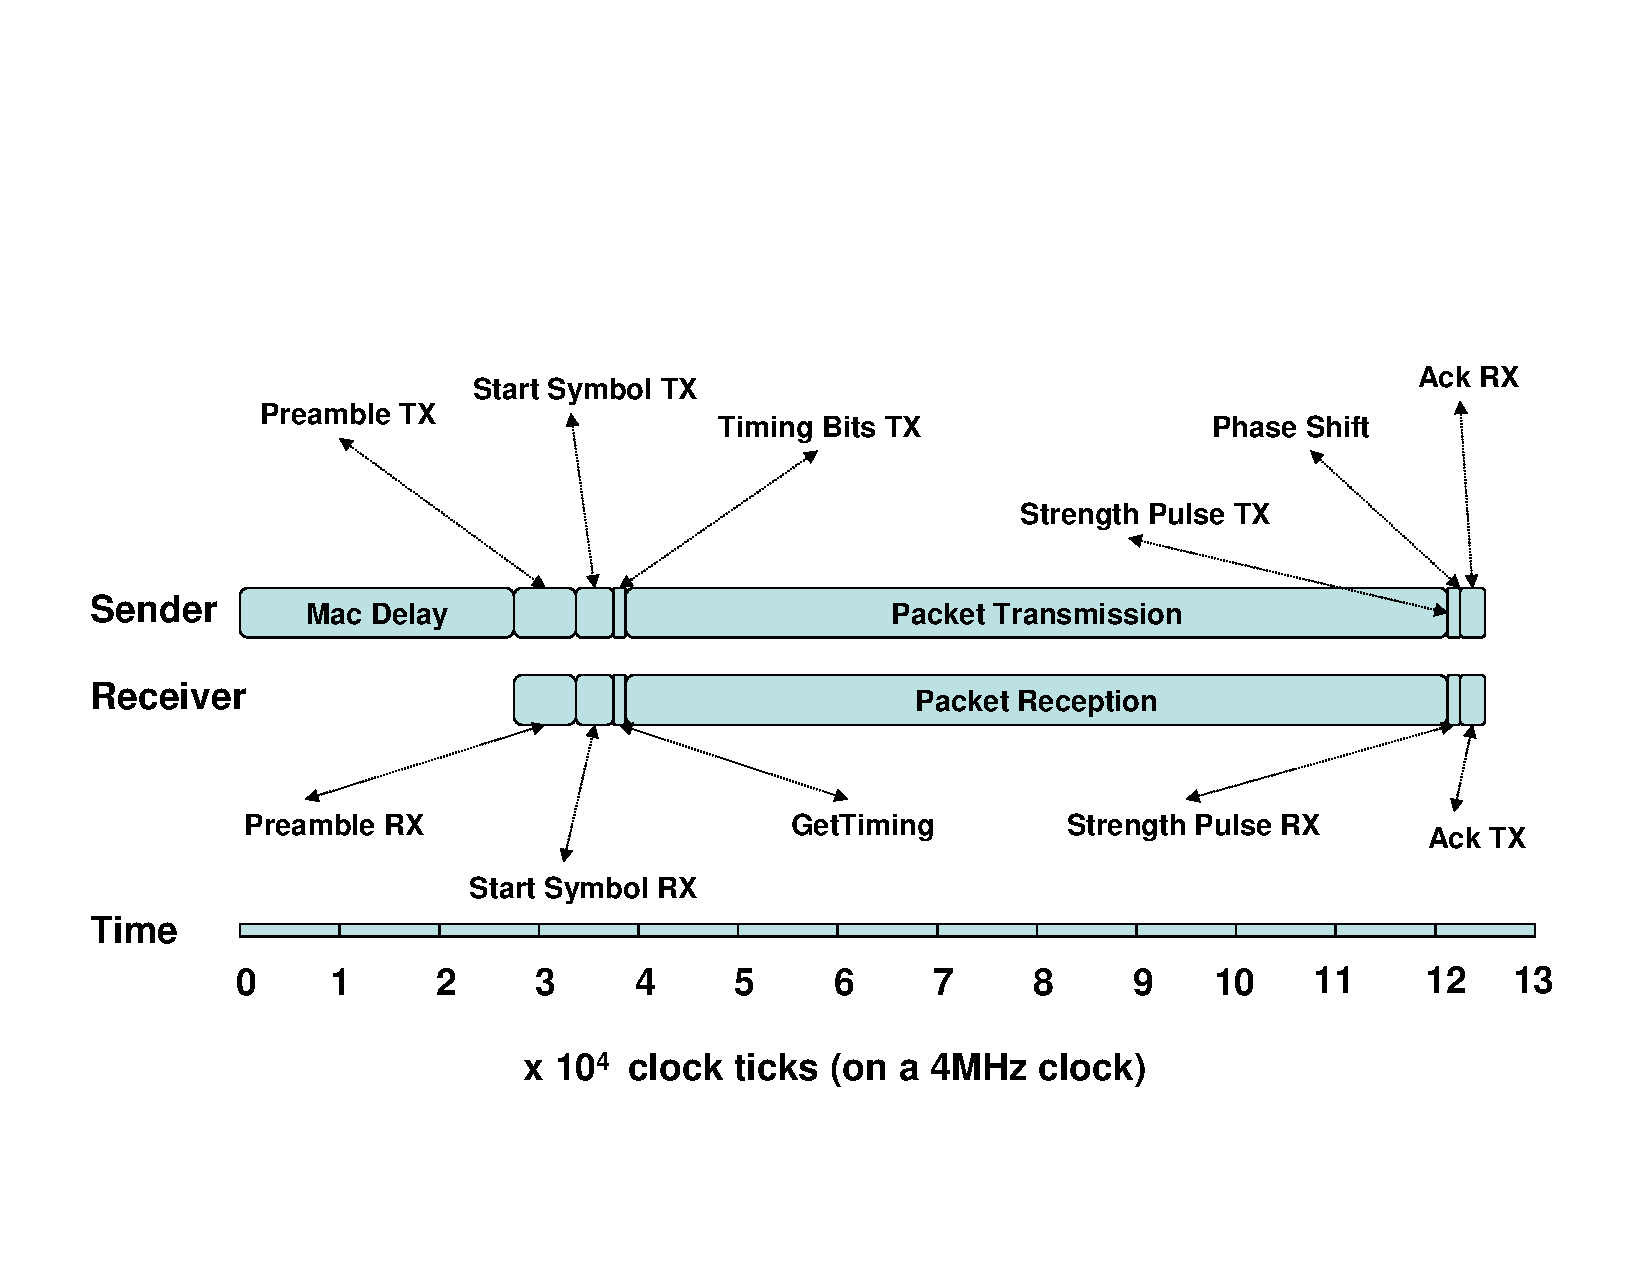
\includegraphics[scale=0.6,angle=-90]{fig/stack.pdf}
\caption{Timing Diagram of Network Send/Receive}
\label{fig:timing}
\end{figure}


\end{document}







